\documentclass{article}
\usepackage[utf8]{inputenc}
\usepackage[spanish]{babel}

% Formato de página
\usepackage[letterpaper, margin = 1.5cm]{geometry}

% Más opciones para enumerar
\usepackage{enumitem}

% Manejo de ecuaciones
\usepackage{amsmath}

% Manejo de imágenes
\usepackage{float}
\usepackage{graphicx}
\usepackage{wrapfig}
\graphicspath{{img/}}

\begin{document}
    \title{
        Fundamentos de bases de datos \\
        Práctica 4 \\
        Modelo Relacional
    }
    \author{
        Díaz Gómez Silvia \\
        Eugenio Aceves Narciso Isaac \\
        Quiroz Castañeda Edgar
    }
    \date {
        22 de marzo del 2019    
    }
    \maketitle
    \section{Modificaciones al esquema}
    \begin{figure}[H]
    	\centering
        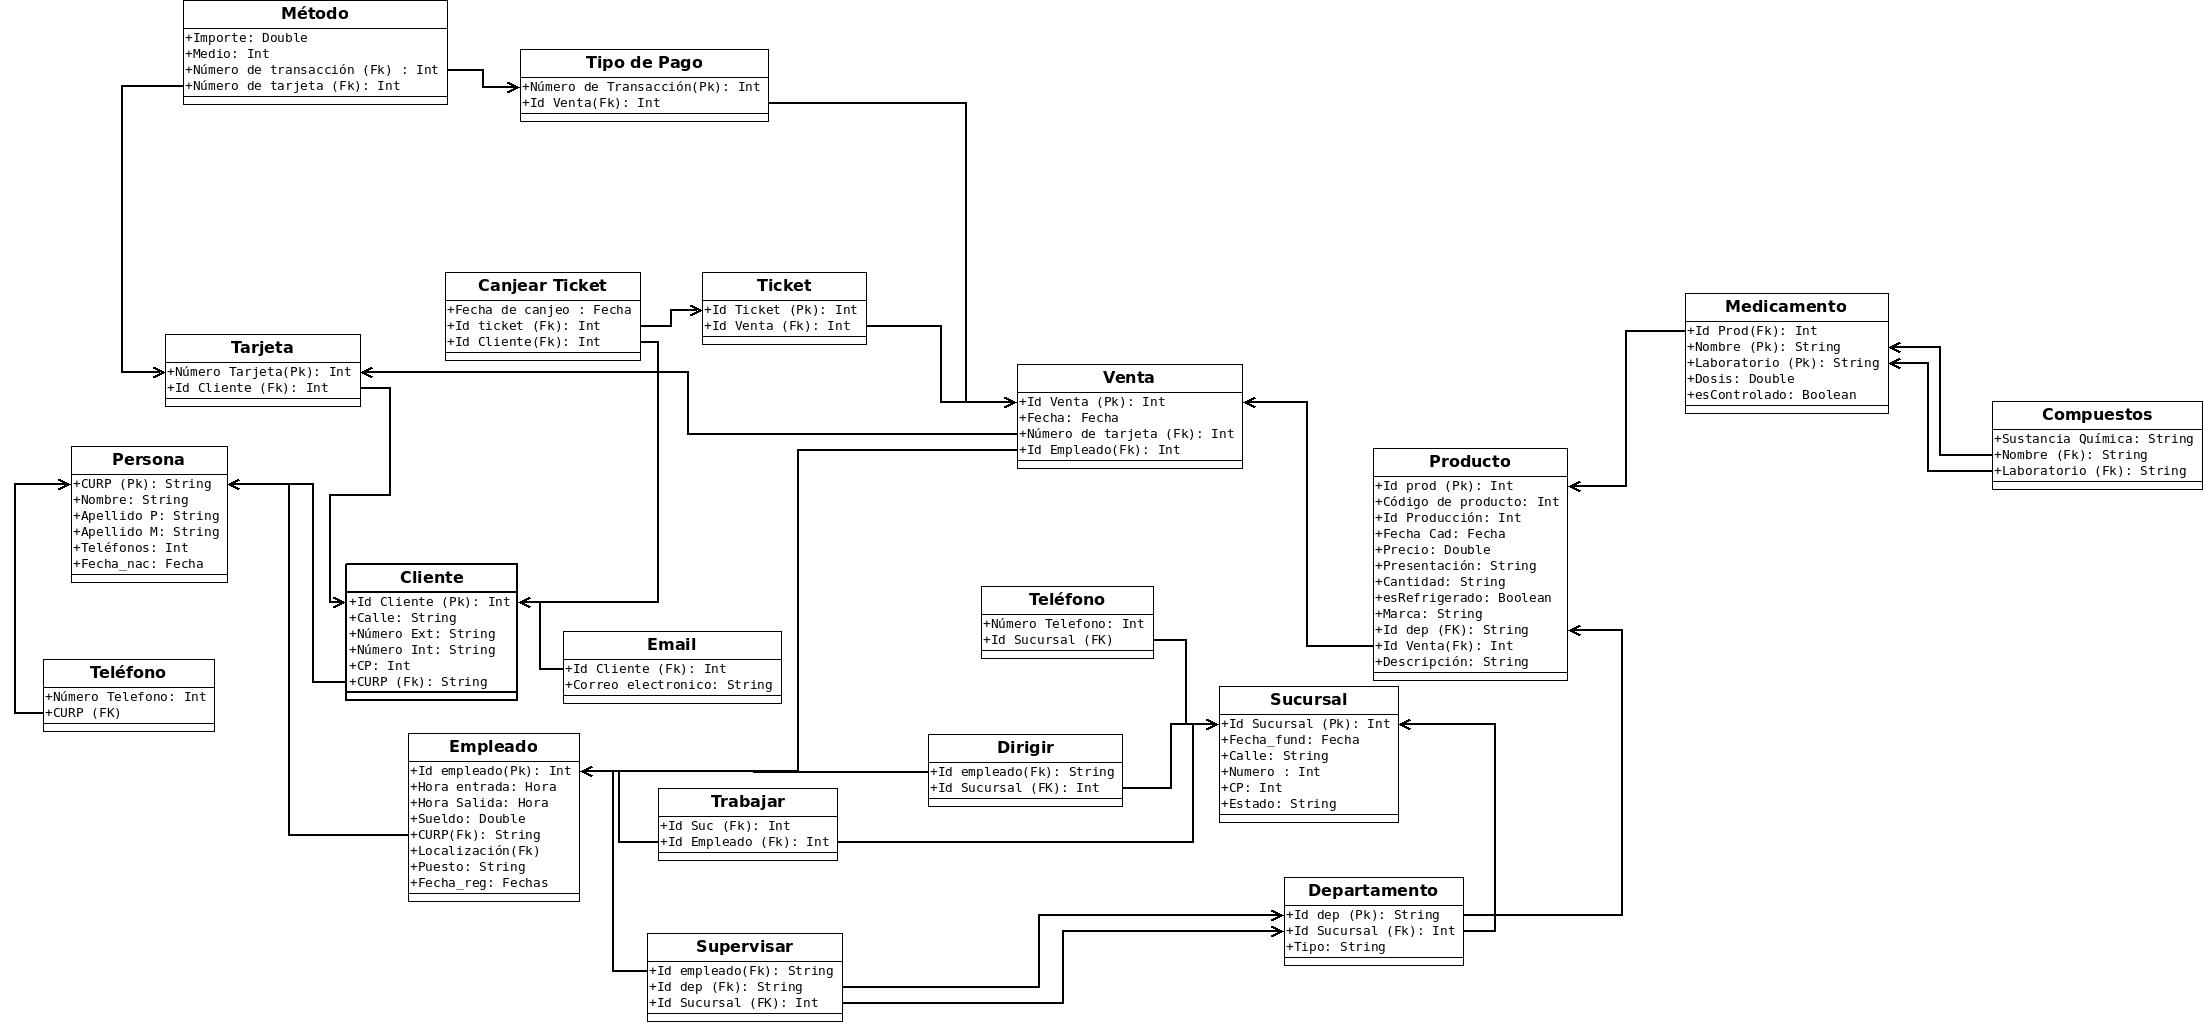
\includegraphics[scale=0.22]{img/practica04.jpeg}
        \caption{Esquema anterior}
    \end{figure}

    \begin{figure}[H]
    	\centering
	  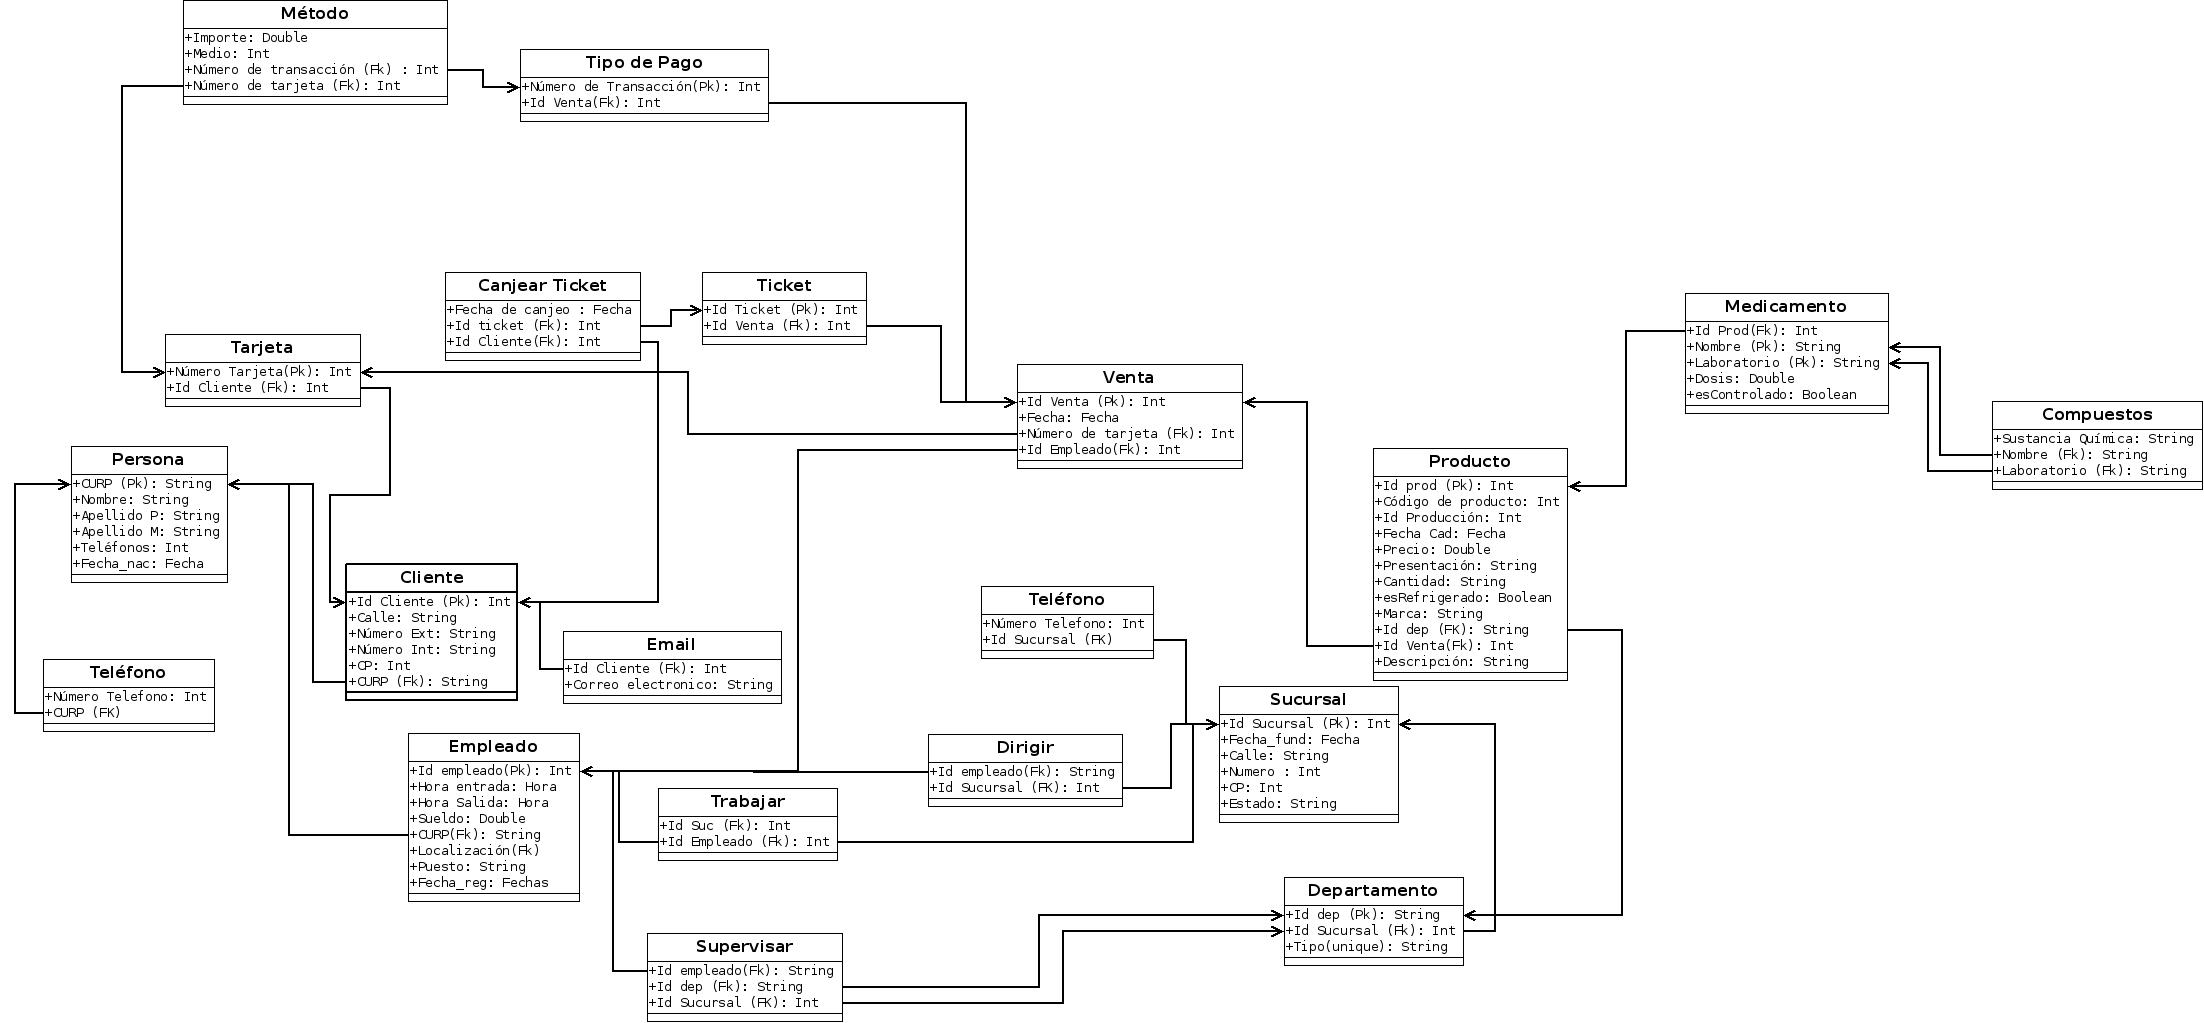
\includegraphics[scale=0.22]{img/practica05.jpeg}
	  \caption{Esquema modificado}
    \end{figure}
    Modificaciones a entidades
    \begin{itemize}
        \item A Empleado se le añaden los atributos de puesto y fecha reg, la
        fecha en la que empezó a trabajar el empleado.
        \item Se cambia el discriminante de Departamento de Localización a Id dep.
        \item A Sucursal se le agrega el atributo de fecha fund, la fecha de 
        establecimiento de esa sucursal.
        \item A Sucursal se le agrean los datos de su dirección, es particular su
        estado.
        \item A Persona se le agrega la fecha nac, la fecha de nacimiento.
        \item A Producto se le agrega el atributo de descr, la descripción. Y 
        se remplaza la llave compuesta por una llave sintética.
        \item En Departamento, el atributo Tipo se vuelve único.
    \end{itemize}

    Modificaciones a relaciones
    \begin{itemize}
        \item Se introduce la tabla de ``Trabajar'' pues es posbile que un
        empleado tenga más de un trabajo.
    \end{itemize}
    
    \section{Álgebra relacional}
    Utilizando el diagrama relacional que haya creado deberán escribir las
    siguientes consultas utilizando los elementos del álgebra relacional.
    \begin{enumerate}
        \item {
            Conocer los datos de las sucursales que tengas más de 15 años
            \begin{align*}
                r &\leftarrow (_{id\_suc}G_{((fecha\_actual-fecha\_reg)/365.25) > 15}(Sucursal)) \\
                %r &\leftarrow \rho_{edad(tiempoDesde(fecha\_reg))}(r) \\
                %r &\leftarrow \sigma_{edad > 15}(r) \\
                %r &\leftarrow r \bowtie Sucursal
            \end{align*}
        }
        \item {
            Conocer el puesto, nombre, edad y la fecha en la que iniciaron a
            trabajar de todos los empleados.
            \begin{align*}
                r &\leftarrow Empleado \bowtie Personas \\
                r &\leftarrow (_{CURP}G_{((fecha\_actual-fecha\_reg)/365.25)}(r))\\
                r &\leftarrow \rho_{edad((fecha\_actual-fecha\_reg)/365.25)}(r) \\
                r &\leftarrow \pi_{nombre, puesto, edad, fech\_reg}(r)
            \end{align*}
        }
        \item {
            Conocer el puesto y edad de todos los empleados que trabajan en más 
            de una sucursal.
            \begin{align*}
                r &\leftarrow (_{id\_empleado}G_{count(id\_empleado)}(Trabajar)) \\
                r &\leftarrow \rho_{num\_trabajos(count(id\_empleado)))}(r)\\
                r &\leftarrow \sigma_{num\_trabajos>1}(r)\\
                r &\leftarrow r \bowtie Empleados \bowtie Persona \\
                r &\leftarrow (_{CURP}G_{((fecha\_actual-fecha\_reg)/365.25)}(r))\\
                r &\leftarrow \rho_{edad((fecha\_actual-fecha\_reg)/365.25)}(r) \\
                r &\leftarrow \pi_{puesto, edad}(r)
            \end{align*}
        }
        \item {
            Conocer los productos que se venden de cada sucursal, para esto se 
            debe regresar el identificador de la sucursal, seguido del
            identificador del producto y la descripción de este.
            \begin{align*}
                r &\leftarrow \pi_{id\_dep, id\_suc}(Departamento \bowtie Sucursal)\\
                r &\leftarrow \pi_{id\_suc, id\_prod, descripcion}(r \bowtie Producto)
            \end{align*}
        }
        \item {
            Conocer los departamentos que tienen cada una de las sucursales.
            \begin{align*}
                r \leftarrow \sigma(Departamento)
            \end{align*}
        }
        \item {
            Conocer cuales son los departamentos que tienene un común todas las 
            sucursales.
            \begin{align*}
                r &\leftarrow (_{tipo}G_{count(Tipo)}(Departamento)) \\
                r &\leftarrow \rho_{num\_tip(count(Tipo))}(r) \\
                g &\leftarrow count_{(id\_suc)}(Sucursal) \\
                r &\leftarrow \sigma_{num\_tip = g}(r)
            \end{align*}
        }
        \item {
            Conocer el cliente más antiguo (el primero en ser registrado, según
            la fecha de registro) en el programa de tarjeta digital de cada una
            de las sucursales registradas.
            \begin{align*}
            r &\leftarrow _{id\_suc,id\_cliente}G_{((fecha\_actual-fecha\_reg)/365.25)}(Clientes \bowtie Sucursal)\\
            r &\leftarrow \rho_{antig((fecha\_actual-fecha\_reg)/365.25)}(r)\\
            r &\leftarrow _{id\_suc,id\_cliente}G_{Max(antig)} (r) \\           
            \end{align*}
        }
        \item {
            Conocer cuáles son los productos que tienen en común cada uno de los
            departamentos de las diferentes sucursales.      
            \begin{align*}
                r &\leftarrow \pi_{id\_suc}(Sucursal) \bowtie
                Departamento \bowtie \pi_{id\dep, id\_prod}(Producto) \\
                numSuc &\leftarrow count(Sucursal) \\
                r &\leftarrow (_{tipo, id\_prod}G_{count(id\_suc)}(r))
                r &\leftarrow \rho_{numSucProd(count(id\_suc))}(r) \\
                r &\leftarrow \sigma_{numSucProd = numSuc}(r)
            \end{align*}
        }
        \item {
            Conocer cuales son TODOS los productos que se tienen en cada uno de
            los departamentos de las diferentes sucursales.
            \begin{align*}
                r \leftarrow Producto
            \end{align*}
        }
        \item {
            Conocer cuál es la sucursal con mayor número de productos
            registrados en sus diferentes departamentos.
            \begin{align*}
            r &\leftarrow _{id\_suc}G_{count(id\_prod)}(Producto \bowtie Departamento)\\
            r &\leftarrow \rho_{cant\_prod(count(id\_prod))}(r)\\
            s &\leftarrow Max_{cant\_prod}(r)\\
            r &\leftarrow \sigma_{cant\_prod=s}(r)\\
            \end{align*}
        }
        \item {
            Eliminar a los empleados que tengan más de 3 trabajos en diferentes 
            sucursales.
            \begin{align*}
                r &\leftarrow (_{id\_empleado}G_{count(id\_empleado)}
                (\pi_{id\_empleado}(Trabajar))) \\
                r &\leftarrow \rho_{num\_trabajos(count(id\_empleado)))}(r)\\
                r &\leftarrow \sigma_{num\_trabajos>3}(r)\\
                r &\leftarrow \pi_{id\_empleado}(r) \bowtie Empleado \\
                Empleado &\leftarrow Empleado - r
            \end{align*}
        }
        \item {
            Eliminar a las sucursales que tengan menos de 1 departamento
            registrado.
            \begin{align*}
                r &\leftarrow \pi_{id\_suc}(Departamento)\\
                r &\leftarrow r \bowtie Sucursal \\
                Sucursal &\leftarrow r
            \end{align*}
        }
        \item {
            Eliminar a los clientes que no hayan utilizado su tarjeta en los
            últimos tres meses.
            \begin{align*}
                r &\leftarrow \pi_{id\_venta, fecha}(Venta) \bowtie TipoDePago \\
                r &\leftarrow \pi_{num\_trans, fecha}(r) \bowtie Metodo \\
                r &\leftarrow \pi_{num\_tarjeta, fecha}(r) \bowtie Tarjeta \\
                r &\leftarrow \pi_{id\_cliente, fecha}(r) \\
                r &\leftarrow (_{id_cliente}G_{max(fecha)}(r)) \\
                r &\leftarrow \rho_{ult\_compra(max(fecha))(r)} \\
                r &\leftarrow \sigma_{ult\_compra/30 > 3}(r) \\
                r &\leftarrow \pi_{id\_cliente}(r) \bowtie Cliente \\
                Cliente &\leftarrow Cliente - r
            \end{align*}
        }
        \item {
            Insertar una nueva sucursal en el estado de México.
            \begin{align*}
                maxId &\leftarrow Max_{id\_suc}(Sucursal)\\
                Sucursal &\leftarrow Sucursal 
                \cup \{(id\_suc = maxId+1, estado='Estado de Mexico', 
                fecha\_fund = hoy)\}
            \end{align*}
        }
        \item {
            Insertar la información de 3 departamentos a la sucursal que fue
            insertada anteriormente.
            \begin{align*}
                id\_s &\leftarrow Max_{id\_suc}(Sucursal)\\
                maxId &\leftarrow Max_{id\_dep}(Departamento)\\
                nSuc &\leftarrow \{(id\_dep = maxId+1, id\_suc=id\_s),
                (id\_dep = maxId+2, id\_suc=id\_s),\\
                &(id\_dep = maxId+3, id\_suc=id\_s)\}\\
                Departamento &\leftarrow Departamento \cup nSuc
            \end{align*}
        }
        \item {
            Actualizar el número de departamentos de la sucursal con menos
            número de éstos, para que ahora tenga la misma cantidad de departamentos
            que la sucursal con mayor números de departamentos.\\
            \textbf{Nota: } Suponemos que tanto el máximo con el mínimo son
            únicos.
            \begin{align*}
                r &\leftarrow (_{id\_suc}G_{count(id\_dep)}(Departamento)) \\
                r &\leftarrow \rho_{num\_dep(count(id\_dep))}(r) \\
                d &\leftarrow max_{num\_dep}(r) \\
                ma &\leftarrow \pi_{id\_suc}(\sigma_{num\_dep=d}(r)) \\
                d &\leftarrow min_{num\_dep}(r) \\
                mi &\leftarrow \pi_{id\_suc}(\sigma_{num\_dep=d}(r)) \\
                dMa &\leftarrow \pi_{tipo}(ma \bowtie Departamento) \\
                dMi &\leftarrow \pi_{tipo}(mi \bowtie Departamento) \\
                depAgr &\leftarrow dMa - dMi \\
                Departamento &\leftarrow Departamento \cup 
                \{(id\_suc=mi, tipo=depAgr)\}
            \end{align*}
        }
    \end{enumerate}

\end{document}